%
% Time-stamp: <2021-01-14 20:59:53 stefan>
%
% ändra alltid i ~/Skrivbord/Arbete/CV/cv.tex
%

\documentclass[a4paper,swedish,10pt]{article}

\usepackage[utf8]{inputenc}
% \usepackage{tgadventor}
\usepackage[scaled=1.1]{gillius2}
\renewcommand*{\familydefault}{\sfdefault}
\usepackage{cinzel}
\usepackage[T1]{fontenc}    %% annars fungerar inte klipp-och-klistra från PDF självt
\usepackage{calc}
\usepackage{babel}
\usepackage[a4paper,top=2cm,bottom=2cm,left=1.5cm,right=1.8cm]{geometry}
% \newcommand{\helv}{\fontfamily{phv}\fontsize{9}{11}\selectfont}
% \usepackage{avant}
% \renewcommand*{\familydefault}{\gilliusfamily}
% \usepackage{mathpazo}

\usepackage{graphicx}
\usepackage[export]{adjustbox}
\usepackage{ragged2e}
\usepackage{enumitem}
\usepackage{blindtext}
\usepackage{adjustbox}
\usepackage[colorlinks=true, allcolors=blue]{hyperref}
\usepackage{fancyhdr}

\setlength{\footskip}{10pt}
\setlength{\headheight}{36pt}
\fancyhf[LH]{Stefan Skoglund\\Högalidsgatan 36\\521 61 Stenstorp}
\fancyhf[CH]{%
  stefan.skoglund@agj.net\\%
  \href{http://www.linkedin.com/in/stefan-niskanen-skoglund-902aa0a1}{Linkedin:Stefan Skoglund}\\
  \href{https://github.com/Skaraborgfakir}{github: Skaraborgfakir}}
\fancyhf[RH]{%
  0500--450 878\\0702--719 835
}
\fancyhf[CF]{\href{https://skaraborgfakir.github.io/cv_minipage.pdf}{Länk till aktuell version}}
\pagestyle{fancy}

\newenvironment*{descriptioncv}[1]%
{%
  \textbf{\Large #1}%
  \begin{description}[nosep,font=\sffamily\bfseries, leftmargin=0.5cm, style=nextline]%
  }%
  {\end{description}\vspace{0.7cm}}
\newcommand*{\cvitem}[3]{\item[#1]{\cinzel#2}\\#3}

% \newenvironment{alignedDescription}[2][0pt]
% {\begin{list}{}%
%   {\renewcommand\makelabel[1]{\textsf{\textbf{##1}}\hfil}%
%   \settowidth\labelwidth{\makelabel{#2}}%
%   \setlength\leftmargin{\labelwidth+\labelsep + #1}}}%
%   {\end{list}}

% DEBUG:utmatning av uppgifter om storlekar,kerning osv
\showoutput
\begin{document}
\hspace{-1.0cm}
\begin{minipage}[t]{0.745\textwidth}
  % \begin{alignedDescription}[10pt]{Het arbete}
  % \item[test]
  % \end{alignedDescription}
  \begin{descriptioncv}{Arbeten}
    \cvitem{Signaltekniker,NVBS}{2017 Maj-- Augusti}{Uthyrd för ny- och ombyggnads-arbeten i samband
      med att Citybanan i Stockholm skulle öppnas. Förberedelser för Getingmidjearbetena.}
    \cvitem{Signaltekniker,NVBS}{2016 Juli}{Uthyrd som sommarvikarie till underhållet vid järnvägen
      i Stockholm.}
    \cvitem{Signaltekniker,NVBS}{2015 Juli-- Augusti}{Uthyrd som sommarvikarie till underhållet
      vid centralstationen (Stockholm.)}
    \cvitem{Tidningsbud,Tidningstjänst}{Juni 2012-- September 2014}{Vikarierande tidningsbud i Stenstorp}
    \cvitem{Servicetekniker,Kronbergs hushållsservice, Skövde}{Mars 1996--November 2006}{reparation av
      vitvaror (spisar,tvättmaskiner och småapparater) och frånluftsvärmepumpar.
      Kundkontakt med planering av arbeten. Försäljning av ersättningsmaskiner. Justering
      av ventilationssystem.}
  \end{descriptioncv}
%  \vspace{0.3cm}
  \begin{descriptioncv}{Utbildningar och separata kurser}
    \cvitem{YH:utbildning,Signaltekniker,Lärcenter i Falköping}{Augusti 2014--Juni 2015}{inriktning
      mot ERTMS, växlar, spårledningar
      vägskydd, ställverk 59 och kommunikation mellan EBISAT och DLC }
    \cvitem{Historia A och B, Göteborgs universitet}{Januari-- December 2018}{Grundkurser i historia, I
      B:uppsatsen använder jag  en Umeåprästs livshistoria som en källa}
    \cvitem{Nordisk välfärdshistoria, Göteborgs universitet}{Våren 2019}{Svensk och norsk 1900:talshistoria,
      hur löste två små länder jämfört med några större olika
      samhällsproblem}
    \cvitem{Skriptprogrammering i Linux, Göteborgs universitet}{Våren 2019}{telemetri med \texttt{awk} och
      \texttt{bash}, del av ett mätteknikprogram vid Chalmers}
    \cvitem{Databasteknik A,Högskolan i Skövde}{2019}{grundläggande databaskonstruktion i MySQL}
    \cvitem{Datornätverk A,Högskolan i Skövde}{2019}{CISCO ICND1}
    \cvitem{Modellering,Högskolan i Skövde}{2018}{UML med grupporienterad verksamhetsmodellering}
    \cvitem{Tyska,Högskolan i Skövde}{2007}{Preparandkurs, gymnasietyska}
  \end{descriptioncv}
 % \vspace{0.5cm}
  \begin{descriptioncv}{Fritidssysslor}
  \item[Ånglokseldare]Aktiv vid museijärnvägsbanan Anten-Gräfsnäs järnväg. Lokeldare sedan 2006
  \item[Ångbåtsaktiv]Matros och eldare ombort på ångbåten Trafik av Hjo
  \item[Studier]Vill kontinuerligt lära mig något nytt om fönsterrenovering, LINUX och IBM MVS
  \end{descriptioncv}
\end{minipage}
\begin{minipage}[t]{0.27\textwidth}
  \raggedleft%
  \vspace{-\topskip}
  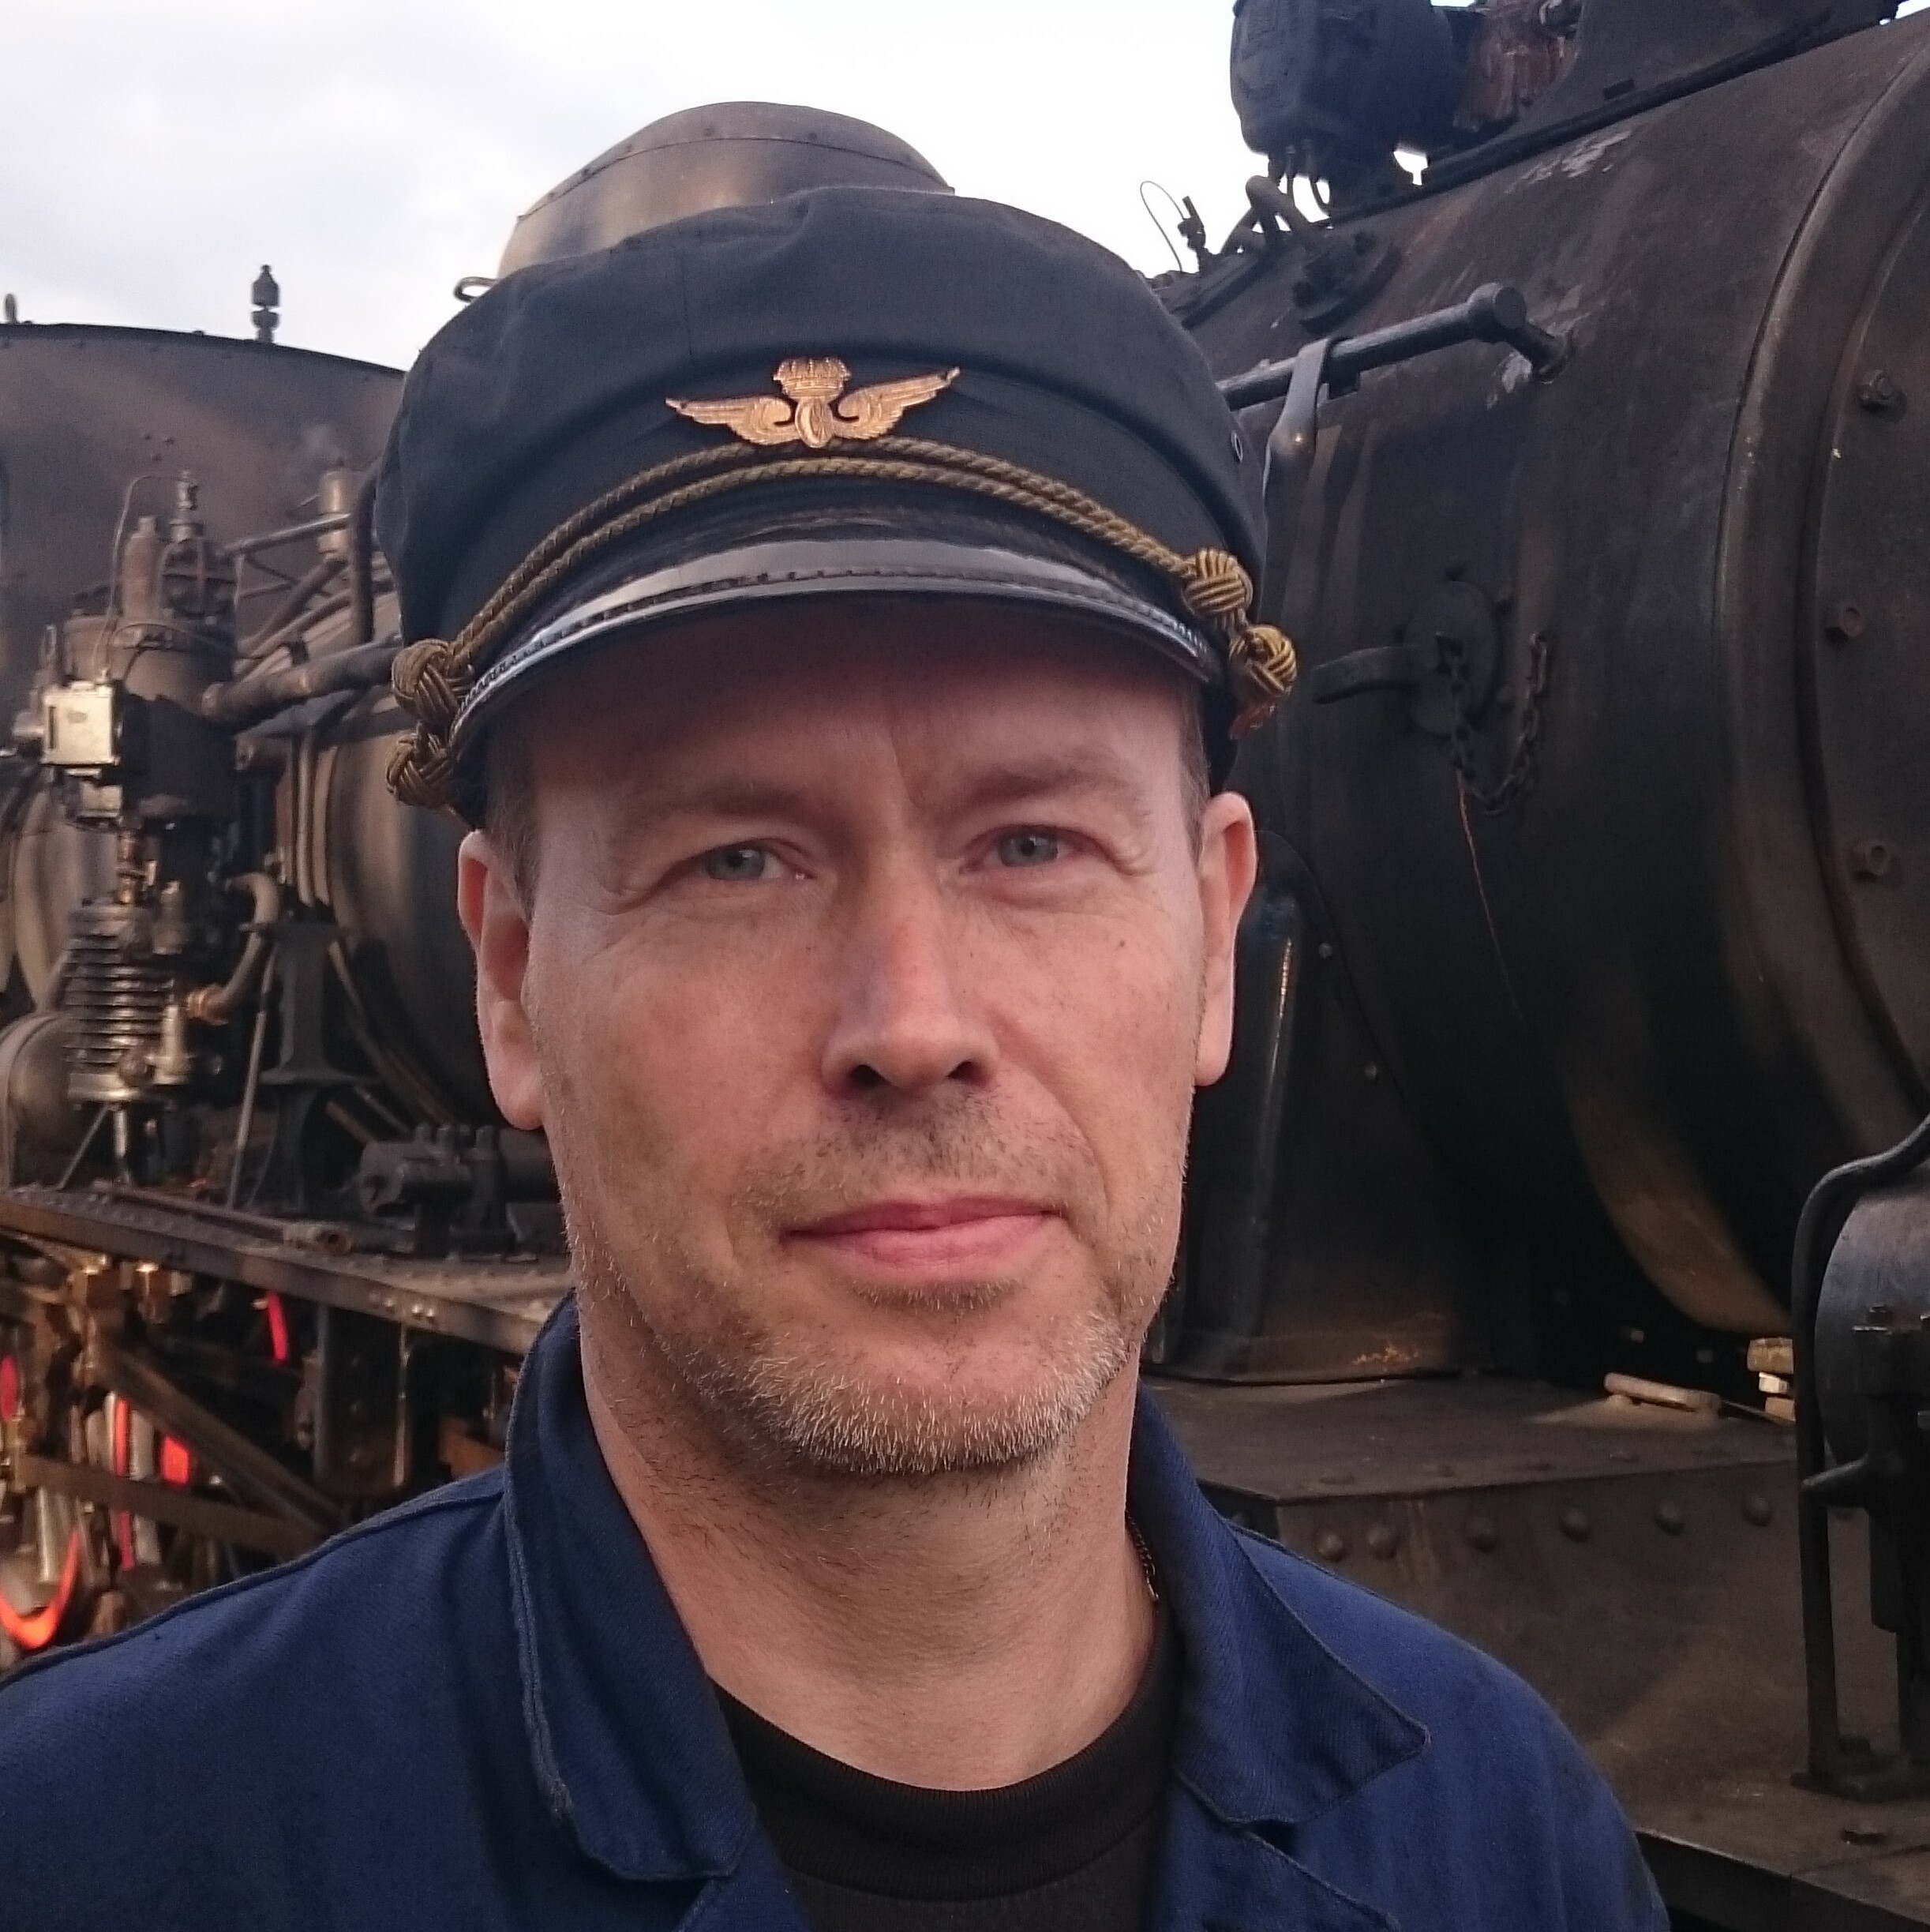
\includegraphics[height=4cm]{bild.jpg}
  \textbf{Utvecklingstekniker}
  \begin{description}[nosep]
    \raggedleft\setlength\itemsep{0.1ex}\small%
  \item Objektorienterad programmering
  \item Människa-Maskin:interaktion
  \item UML
  \item C/C++
  \item Pascal
  \end{description}
  \vspace{0.5cm}
  \textbf{IT:kunskaper}
  \begin{description}[nosep]
    % \setlength{\labelwidth}{0ex}
    % \setlength{\leftmargin}{0ex}
    % \setlength{\labelsep}{0ex}
    % \setlength{\itemindent}{1\parindent}
    % \setlength{\listparindent}{1\parindent}
    % \setlength{\itemsep}{0ex}
    % \setlength{\topsep}{\dimexpr-\parskip-\baselineskip}
    % \setlength{\parsep}{0ex}
    % \setlength{\partopsep}{0ex}
    \raggedleft\setlength\itemsep{0.1ex}\small%
  \item CFEngine
  \item LINUX
  \item Solaris
  \item Microsoft Word
  \item OpenLDAP
  \item MySQL
  \item PostgreSQL
  \item Datornätverk
  \item Automatisering av PKI
  \item MVS (nybörjare)
  \end{description}
  \vspace{0.5cm}
  \textbf{Språk}
  \begin{description}[nosep,itemsep=0.1ex]
    \raggedleft\small%
  \item Svenska (modersmål)
  \item Engelska (van, samtal och skriftlig)
  \item Tyska (nybörjare)
  \end{description}
  \vspace{0.5cm}
  \textbf{Behörigheter}
  \begin{description}[nosep]
    \raggedleft\setlength\itemsep{0.1ex}\small%
  \item B:körkort
  \item Skydds- och säkerhetsledare
  \item HLR
  \end{description}
  \vspace{5cm}
  \textbf{Colophon}
  \begin{description}[nosep]
    \raggedleft\setlength\itemsep{0.1ex}\small%
  \item Stefan Skoglund {\cinzel{2021}}
  \item Gillius
  \item Cinzel (årtal)
  \item \LaTeX%
  \end{description}
\end{minipage}

% \begin{description}
%   \setlength\itemsep{0.1cm}
%   \begin{FlushRight}
%   \item Persona design
%   \item Heuristic eval
%   \end{FlushRight}
% \end{description}

% \textbf{Personlighet}%
% \begin{description}%
%     %   \setlength\itemsep{0.1cm}
% \item Läraktigt
% \item Metodisk
% \item Noggrann
% \item Seriös
% \end{description}
% \textbf{IT:kunskaper}
% \begin{itemize}
%   \setlength\itemsep{1.0em}
% \item Fortran
% \item ML
% \item LISP
% \item CFEngine
% \item FrameMaker
% \item Adobe CS
% \end{itemize}
% \end{flushright}

\end{document}

%%% Local Variables:
%%% mode: latex
%%% End:
